\documentclass[11pt, a4paper]{article}
\usepackage{graphicx}
\usepackage{amsmath}
\usepackage{listings}
\usepackage{color}
\usepackage{fancyhdr}
\usepackage[utf8]{inputenc}
\usepackage[%  
    colorlinks=true,
    pdfborder={0 0 0},
    linkcolor=red
]{hyperref}

\definecolor{dkgreen}{rgb}{0,0.6,0}
\definecolor{gray}{rgb}{0.5,0.5,0.5}
\definecolor{mauve}{rgb}{0.58,0,0.82}

\lstset{frame=tb,
  language=Python,
  aboveskip=3mm,
  belowskip=3mm,
  showstringspaces=false,
  columns=flexible,
  basicstyle={\small\ttfamily},
  numbers=none,
  numberstyle=\tiny\color{gray},
  keywordstyle=\color{blue},
  commentstyle=\color{dkgreen},
  stringstyle=\color{mauve},
  breaklines=true,
  breakatwhitespace=true,
  tabsize=3
}



\title{EE2703-Assignment4}
\author{EE19B094 }
\date{March 2021}

\setlength{\headheight}{15pt}
\pagestyle{fancy}
\fancyhf{}
\rhead{Assignment - 4}
\lhead{EE2703 - Applied Programming Lab}
\rfoot{Page \thepage}

\begin{document}

\maketitle
\newpage

\begin{abstract}
     The purpose of this assignment is to find fourier series coefficients of two curves 1) $e^x$ and 2) $cos(cos(x))$. We will use two different methods to calculate the fourier coefficients and find the error between the methods.
\end{abstract}




\section{Introduction}
\par The Fourier Series of a function $f(x)$ with period $2\pi$ is computed as follows:
\begin{equation}
    f(x) = a_0 + \sum_{n=1}^{+\infty}\{ a_ncos(nx) +b_nsin(nx)\}
\end{equation}
\newline
where , \newline

\begin{equation}
    a_0 = \frac{1}{2\pi} \int_0^{2\pi}f(x)dx\\
\end{equation}
\begin{equation}
    a_n = \frac{1}{2\pi} \int_0^{2\pi}f(x)*\cos(nx)dx
\end{equation}
\begin{equation}
    b_n = \frac{1}{2\pi} \int_0^{2\pi}f(x)*\sin(nx)dx\\
\end{equation}
    
Now, as $e^x$ doesn't have a period of $2\pi$, We will change its definition in a way that will make it periodic i.e. we extend the function from [0,$2\pi$) to ($-\infty,\infty$).



\section{Generating and plotting raw functions}
\par We can generate the functions using the \emph{Numpy} library. The x values range from [-4$\pi$,2$\pi$]. Remember that we extended the $e^x$ function as it was not periodic and thus it is calculated as $e^{x\%(2\pi)}$ thus making it periodic with period 2$\pi$.

\begin{lstlisting}
generate_exp = lambda x: np.exp(x)  #Function to generate aperodic e^x function
generate_coscos = lambda x: np.cos(np.cos(x))   #Function to generate cos(cos(x)) function
generate_perodic_exp = lambda x: np.exp(x%(2*math.pi))  #Function to generate periodic e^x function


#Function to plot both kind of exponential functions
def plot_raw_exponential():
    x = np.linspace(-2*math.pi,4*math.pi,300)     
    figure(1)
    semilogy(x,generate_exp(x),'m',label=r'Aperiodic $e^x$ in log scale')      
    semilogy(x,generate_perodic_exp(x),'g',label=r'Periodically extended $e^x$ in log scale')
    title("Q1 : Plotting original functions")
    xlabel(r'$x\longrightarrow$',fontsize=12)
    ylabel(r'$log(e^{x})\longrightarrow$',fontsize=12)
    grid()
    legend()
    savefig("Q1-1.png")
    close()

#Function to plot cos(cos(x)) function
def plot_raw_coscosx():
    x = np.linspace(-2*np.pi,4*np.pi,300)
    figure(2)
    plot(x,generate_coscos(x))
    title(r'y = cos(cos(x))')
    xlabel(r'$x\longrightarrow$', fontsize = 12)
    ylabel(r'$cos(cos(x))\longrightarrow$', fontsize = 12)
    grid()
    savefig("Q1-2.png")
    close()

plot_raw_exponential()     #Q1 plots function call
plot_raw_coscosx()
\end{lstlisting}
\par  Graphs below show the aperiodic and periodic versions of $e^x$ in log scale and $cos(cos(x))$ in linear scale.

\begin{figure}[!tbh]
    \centering
    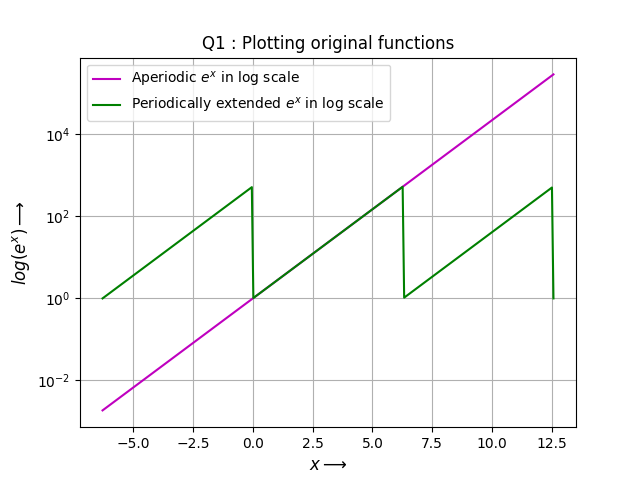
\includegraphics[scale = 0.7]{Q1-1.png}
    \caption{$e^x$}
    \label{fig:Figure 1}
\end{figure}

\begin{figure}[!tbh]
    \centering
    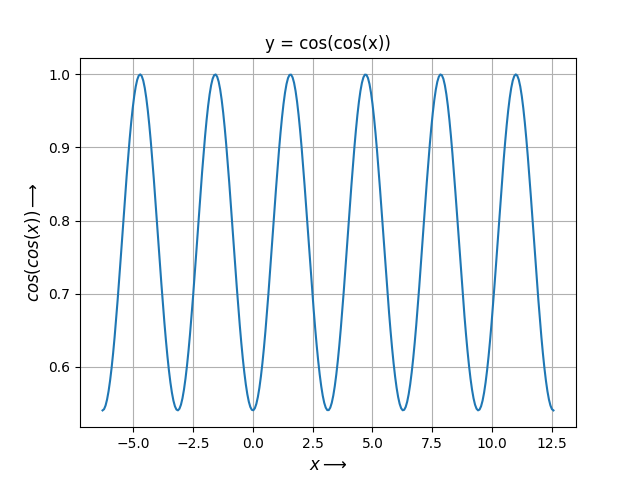
\includegraphics[scale = 0.7]{Q1-2.png}
    \caption{$cos(cos(x))$}
    \label{fig:Figure 2}
\end{figure}


\newpage
\section{Fourier Series Coefficients calculation}
\par We create two new functions to be integrated, namely \begin{verbatim}
    u(x,k)=f(x)*cos(kx)
\end{verbatim} and
\begin{verbatim}
    v(x,k)=f(x)*sin(kx)
\end{verbatim}
We obtain the first 25 co-efficients for both $e^x$ and $cos(cos(x))$ by using the equations given in the introduction, scipy’s built in integrator and the quad function to pass extra arguments to the function being integrated. They are stored in a vector in the order
\begin{center}
     $
    \begin{pmatrix}
    a_0\\
    a_1\\
    b_1\\
    ...\\
    a25\\
    b25\\
    \end{pmatrix}
     $
    
\end{center}
\begin{lstlisting}
#Function to calculate 'k' Fourier Coefficients for given function f
def calculate_fourier_coefficients(f,k):                       
    coeffs=[]   #List storing combined coefficients
    a_n=[]      #List storing a_n coefficients
    b_n=[]      #List storing b_n coefficients
                            
    u = lambda x, n: f(x)*math.cos(n*x)     #Functions to be integrated
    v = lambda x, n: f(x)*math.sin(n*x)
                                                                        
    a_n.append((1/(2*math.pi))*integ.quad(u, 0, 2*math.pi, args=0)[0])      #a_0
    coeffs.append((1/(2*math.pi))*integ.quad(u, 0, 2*math.pi, args=0)[0])
    b_n.append(0) 

    for n in range(1,k):
        a_n.append((1/math.pi)*integ.quad(u, 0, 2*math.pi, args=n)[0])    
        coeffs.append((1/math.pi)*integ.quad(u, 0, 2*math.pi, args=n)[0])
        
        b_n.append((1/math.pi)*integ.quad(v, 0, 2*math.pi, args=n)[0])   
        coeffs.append((1/math.pi)*integ.quad(v, 0, 2*math.pi, args=n)[0]) 
    
    return coeffs,a_n,b_n

#Calculating fourier coefficients using integration method
coeffs_exp,a_n_exp,b_n_exp = calculate_fourier_coefficients(generate_exp,COEFF_COUNT+1)
coeffs_coscos,a_n_coscos,b_n_coscos = calculate_fourier_coefficients(generate_coscos,COEFF_COUNT+1)
\end{lstlisting}


\section{Plotting the Fourier Coefficients}
\par We plot all the fourier coefficients for both the functions on two scales i.e. loglog and semilog.
\begin{lstlisting}
    #Function to plot the coefficients
def plot_coefficients():
    #Coefficients of e^x on a log scale
    figure(3)
    semilogy(np.abs(a_n_exp),'ro',label=r'$a_n$ of $e^x$')
    semilogy(np.abs(b_n_exp),'bo',label=r'$b_n$ of $e^x$')    
    grid(True)
    title(r'Magnitudes of coefficients in log scale', fontsize = 10)
    xlabel(r'n$\longrightarrow$')
    ylabel(r'log(coeffs)$\longrightarrow$')
    legend()
    savefig("Q3-1.png")
    close()
    
    #Coefficients of cos(cos(x)) on a log scale
    figure(4)
    semilogy(np.abs(a_n_coscos),'ro',label=r'$a_n$ of $cos(cos(x))$')
    semilogy(np.abs(b_n_coscos),'bo',label=r'$b_n$ of $cos(cos(x))$')
    grid(True)
    title(r'Magnitudes of coefficients in log scale', fontsize = 10)
    xlabel(r'n$\longrightarrow$')
    ylabel(r'log(coeff)$\longrightarrow$')
    legend()
    savefig("Q3-2.png")
    close()
    
    #Coefficients of e^x on a loglog scale
    figure(5)
    loglog(np.abs(a_n_exp),'ro',label=r'$a_n$ of $e^x$')
    loglog(np.abs(b_n_exp),'bo',label=r'$b_n$ of $e^x$')
    grid(True)
    title(r'Magnitudes of coefficients in loglog scale', fontsize = 10)
    xlabel(r'n$\longrightarrow$')
    ylabel(r'log(log(coeff))$\longrightarrow$')
    legend()
    savefig("Q3-3.png")
    close()
    
    #Coefficients of cos(cos(x)) on a loglog scale
    figure(6)
    loglog(np.abs(a_n_coscos),'ro',label=r'$a_n$ of $cos(cos(x))$')
    loglog(np.abs(b_n_coscos),'bo',label=r'$b_n$ of $cos(cos(x))$')
    grid(True)
    title(r'Magnitudes of coefficients in loglog scale', fontsize = 10)
    xlabel(r'n$\longrightarrow$')
    ylabel(r'log(log(coeff))$\longrightarrow$')
    legend()
    savefig("Q3-4.png")
    close()

plot_coefficients()
\end{lstlisting}
\begin{figure}[!tbh]
    \centering
    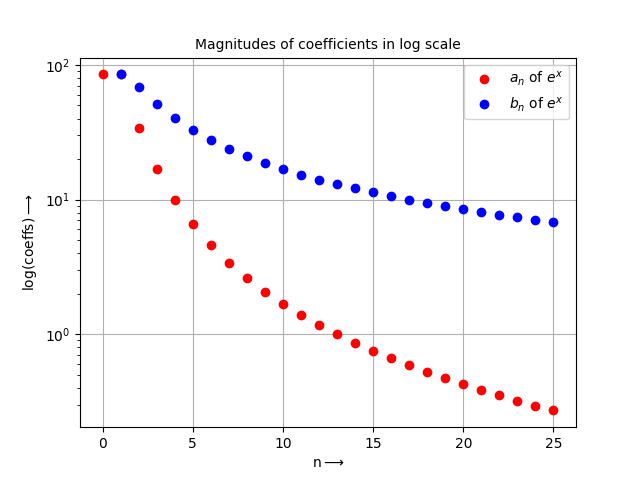
\includegraphics[scale = 0.7]{Q3-1.png}
    \caption{$e^x\ in\ log\ scale$}
    \label{fig:Figure 3}
\end{figure}

\begin{figure}[!tbh]
    \centering
    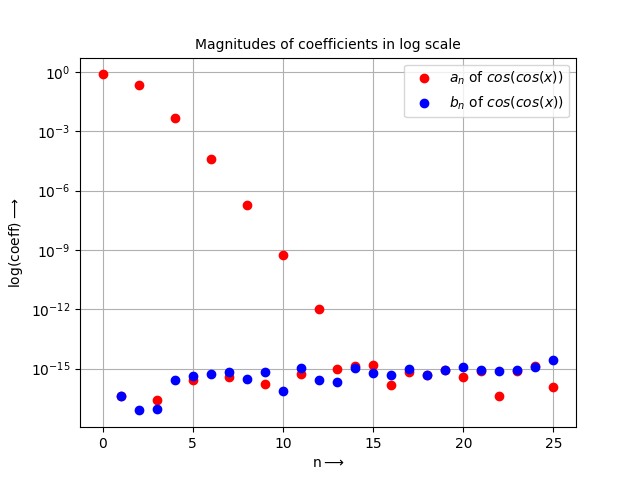
\includegraphics[scale = 0.7]{Q3-2.png}
    \caption{$cos(cos(x))\ in\ log\ scale$}
    \label{fig:Figure 4}
\end{figure}

\begin{figure}[!tbh]
    \centering
    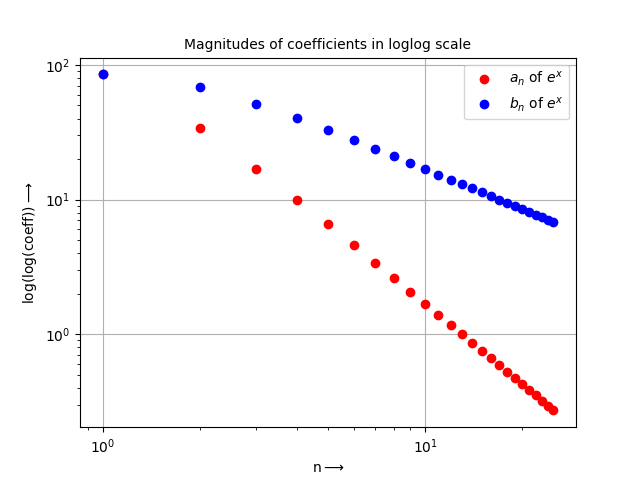
\includegraphics[scale = 0.7]{Q3-3.png}
    \caption{$e^x\ in\ loglog\ scale$}
    \label{fig:Figure 5}
\end{figure}

\begin{figure}[!tbh]
    \centering
    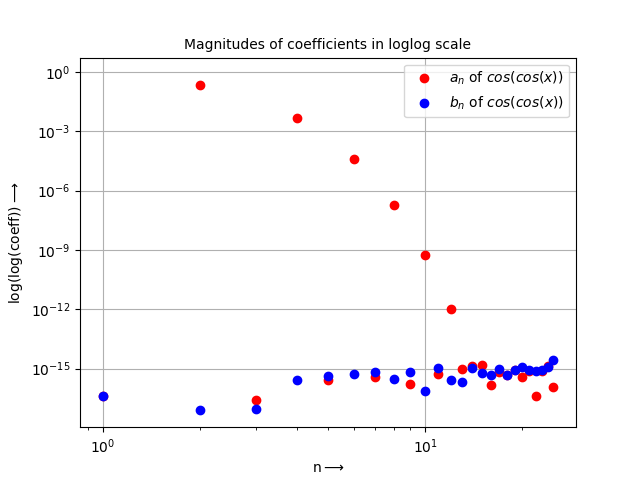
\includegraphics[scale = 0.7]{Q3-4.png}
    \caption{$cos(cos(x))\ in\ loglog\ scale$}
    \label{fig:Figure 6}
\end{figure}


\newpage
\section{Observations}
\textbf{Q :} The $b_n$ coefficients for $cos(cos(x))$ are nearly approaching zero in Figure \ref{fig:Figure 4}. What is the reason ?\newline
\textbf{A :} As $cos(cos(x))$ is an even function, its fourier series will be a pure cosine series with no sine terms i.e. $b_n=0$. \newline \newline

\noindent\textbf{Q :} The coefficients for $cos(cos(x))$ decrease rapidly as compared to $e^x$ for higher frequencies. Why ?\newline
\textbf{A :} $cos(cos(x))$ is a sinusoid type of function and thus most of the contribution is from the lower frequencies. And therefore the values of coefficients decreases rapidly for higher frequencies. This is evident from Figure \ref{fig:Figure 4}. Whereas $e^x$ has contributions from many harmonics due to the discontinuities in our periodic definition of $e^x$ and thus it's coefficients decrease less rapidly. This can be seen in Figure \ref{fig:Figure 3}.\newline\newline

\noindent\textbf{Q :} Why does the loglog plot of Figure \ref{fig:Figure 5} look linear while the log plot of Figure \ref{fig:Figure 4} look linear ?\newline
\textbf{A :} The coefficients of $e^x$ decay with n as\\ \begin{center}
    $a_n \propto 1/n^2$\\ $b_n \propto 1/n$ 
\end{center} hence, taking log, $\log a_n$ and $\log b_n$ are almost proportional to log(n). So the loglog scale features linear behaviour. For cos(cos(x)) the FSC’s decay approximately exponentially with n i.e \begin{center}
    $a_n , b_n \propto e^{-n}$
\end{center}, and hence the log plot looks linear.



\section{Least Square Approach}
We will now try and predict the values of fourier coefficients using the least square approach. We will create two matrices $A,x$ satisfying the equation 
\begin{center}
    $A\begin{pmatrix}
    a_0\\
    a_1\\
    b_1\\
    ...\\
    a25\\
    b25\\
    \end{pmatrix} = x$ \\
\end{center}
    $\begin{pmatrix}
    1 & cos(x_1) & sin(x_1) & ... & cos(25x_1) & sin(25x_1) \\
    1 & cos(x_2) & sin(x_2) & ... & cos(25x_2) & sin(25x_2) \\
    ... & ... & ... & ... & ... & ...\\
    1 & cos(x_{400}) & sin(x_{400}) & ... & cos(25x_{400}) & sin(25x_{400}) \\
    \end{pmatrix}
    \begin{pmatrix}
    a_0\\
    a_1\\
    b_1\\
    ...\\
    a25\\
    b25\\
    \end{pmatrix} =$
    $\begin{pmatrix}
    f(x_1)\\
    f(x_2)\\
    ...\\
    f(x_{400})
    \end{pmatrix} $\newline
Now, using \emph{scipy.linalg.lstsq()} function, we find the coefficient matrix.\newline
\begin{lstlisting}
#Defining A,x arrays for lstsq method
x = np.linspace(0,2*pi,401)
x=x[:-1]  
A = np.zeros((400,2*COEFF_COUNT+1)) 
A[:,0]=1 
for k in range(1,COEFF_COUNT+1):
    A[:,2*k-1] = np.cos(k*x) 
    A[:,2*k] = np.sin(k*x) 

 
#Calculating coefficients for e^x using lstsq method
coeffs_exp_lstsq = scipy.linalg.lstsq(A,generate_exp(x))[0] #List storing combined coefficients
a_n_exp_lstsq = []  #List storing a_n coefficients
b_n_exp_lstsq = []  #List storing b_n coefficients

#Deriving a_n and b_n from combined coefficients
a_n_exp_lstsq.append(coeffs_exp_lstsq[0])
b_n_exp_lstsq.append(0)
for i in range(1,2*COEFF_COUNT+1,2):
    a_n_exp_lstsq.append(coeffs_exp_lstsq[i])
for i in range(2,2*COEFF_COUNT+1,2):
    b_n_exp_lstsq.append(coeffs_exp_lstsq[i])


#Calculating coefficients for cos(cos(x)) using lstsq method
coeffs_coscos_lstsq = scipy.linalg.lstsq(A,generate_coscos(x))[0] #List storing combined coefficients
a_n_coscos_lstsq = []   #List storing a_n coefficients
b_n_coscos_lstsq = []   #List storing b_n coefficients

#Deriving a_n and b_n from combined coefficients
a_n_coscos_lstsq.append(coeffs_coscos_lstsq[0])
b_n_coscos_lstsq.append(0)
for i in range(1,2*COEFF_COUNT+1,2):
    a_n_coscos_lstsq.append(coeffs_coscos_lstsq[i])
for i in range(2,2*COEFF_COUNT+1,2):
    b_n_coscos_lstsq.append(coeffs_coscos_lstsq[i])
\end{lstlisting}
\par The below shown graphs show the difference in values of coefficients calculated using the two methods.

\begin{lstlisting}
    #Plot coefficients obtained from integration and lstsq methods
def plot_comparing_coeff():
    #Coefficients of e^x on a log scale
    figure(7)
    fig, axs = plt.subplots(2)
    axs[0].semilogy(np.abs(a_n_exp_lstsq), 'bo', label = 'Least Squares Approach')
    axs[0].semilogy(np.abs(a_n_exp), 'go', label = 'Integration Approach')
    axs[1].semilogy(np.abs(b_n_exp_lstsq), 'bo', label = 'Least Squares Approach')
    axs[1].semilogy(np.abs(b_n_exp), 'go', label = 'Integration Approach')
    fig.suptitle(r'Magnitudes of coefficients in log scale for e^x')
    axs[0].set(ylabel=r'log(|$a_n$|)$\longrightarrow$',xlabel=r'$n\longrightarrow$')
    axs[1].set(ylabel=r'log(|$b_n$|)$\longrightarrow$',xlabel=r'$n\longrightarrow$')
    axs[0].grid()
    axs[1].grid()
    axs[0].legend()
    axs[1].legend()
    savefig("Q5-1.png")
    close()

    #Coefficients of cos(cos(x)) on a log scale
    figure(8)
    fig, axs = plt.subplots(2)
    axs[0].semilogy(np.abs(a_n_coscos_lstsq), 'bo', label = 'Least Squares Approach')
    axs[0].semilogy(np.abs(a_n_coscos), 'go', label = 'Integration Approach')
    axs[1].semilogy(np.abs(b_n_coscos_lstsq), 'bo', label = 'Least Squares Approach')
    axs[1].semilogy(np.abs(b_n_coscos), 'go', label = 'Integration Approach')
    fig.suptitle(r'Magnitudes of coefficients in log scale for cos(cos(x))')
    axs[0].set(ylabel=r'log(|$a_n$|)$\longrightarrow$',xlabel=r'$n\longrightarrow$')
    axs[1].set(ylabel=r'log(|$b_n$|)$\longrightarrow$',xlabel=r'$n\longrightarrow$')
    axs[0].grid()
    axs[1].grid()
    axs[0].legend()
    axs[1].legend()
    savefig("Q5-2.png")
    close()

    #Coefficients of e^x on a loglog scale
    figure(9)
    fig, axs = plt.subplots(2)
    axs[0].loglog(np.abs(a_n_exp_lstsq), 'bo', label = 'Least Squares Approach')
    axs[0].loglog(np.abs(a_n_exp), 'go', label = 'Integration Approach')
    axs[1].loglog(np.abs(b_n_exp_lstsq), 'bo', label = 'Least Squares Approach')
    axs[1].loglog(np.abs(b_n_exp), 'go', label = 'Integration Approach')
    fig.suptitle(r'Magnitudes of coefficients in log scale for e^x')
    axs[0].set(ylabel=r'log(|$a_n$|)$\longrightarrow$',xlabel=r'$n\longrightarrow$')
    axs[1].set(ylabel=r'log(|$b_n$|)$\longrightarrow$',xlabel=r'$n\longrightarrow$')
    axs[0].grid()
    axs[1].grid()
    axs[0].legend()
    axs[1].legend()
    savefig("Q5-3.png")
    close()

    #Coefficients of cos(cos(x)) on a loglog scale
    figure(10)
    fig, axs = plt.subplots(2)
    axs[0].loglog(np.abs(a_n_coscos_lstsq), 'bo', label = 'Least Squares Approach')
    axs[0].loglog(np.abs(a_n_coscos), 'go', label = 'Integration Approach')
    axs[1].loglog(np.abs(b_n_coscos_lstsq), 'bo', label = 'Least Squares Approach')
    axs[1].loglog(np.abs(b_n_coscos), 'go', label = 'Integration Approach')
    fig.suptitle(r'Magnitudes of coefficients in log scale for cos(cos(x))')
    axs[0].set(ylabel=r'log(|$a_n$|)$\longrightarrow$',xlabel=r'$n\longrightarrow$')
    axs[1].set(ylabel=r'log(|$b_n$|)$\longrightarrow$',xlabel=r'$n\longrightarrow$')
    axs[0].grid()
    axs[1].grid()
    axs[0].legend()
    axs[1].legend()
    savefig("Q5-4.png")
    close()

plot_comparing_coeff()  #Q5 plots function call
\end{lstlisting}
\begin{figure}[!tbh]
    \centering
    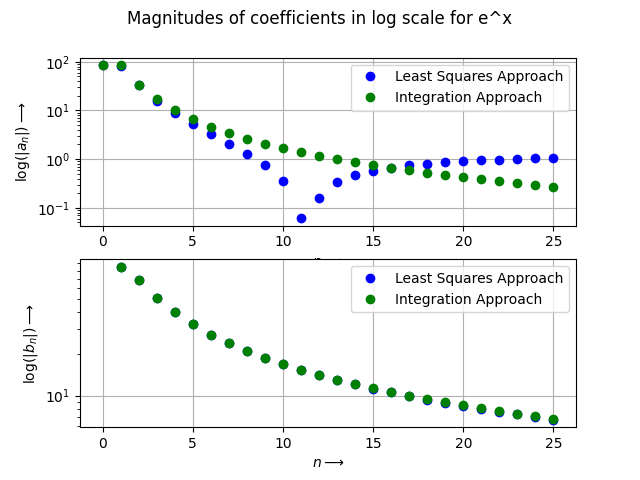
\includegraphics[scale = 0.7]{Q5-1.png}
    \caption{$e^x\ in\ log\ scale$}
    \label{fig:Figure 7}
\end{figure}
\begin{figure}
    \centering
    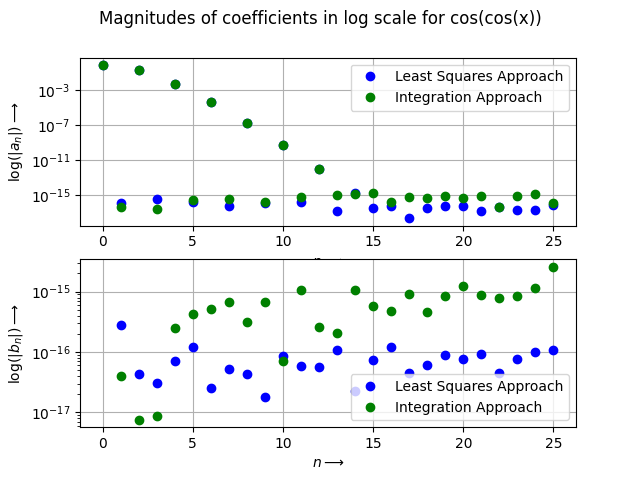
\includegraphics[scale = 0.7]{Q5-2.png}
    \caption{$cos(cos(x))\ in\ log\ scale$}
    \label{fig:Figure 8}
\end{figure}
\begin{figure}
    \centering
    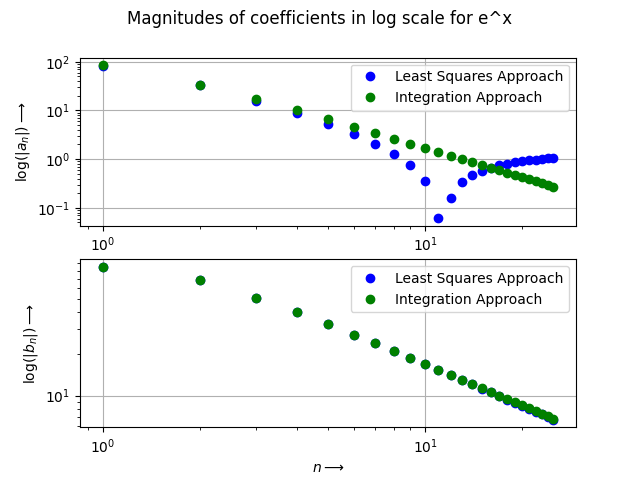
\includegraphics[scale = 0.7]{Q5-3.png}
    \caption{$e^x\ in\ loglog\ scale$}
    \label{fig:Figure 9}
\end{figure}
\begin{figure}
    \centering
    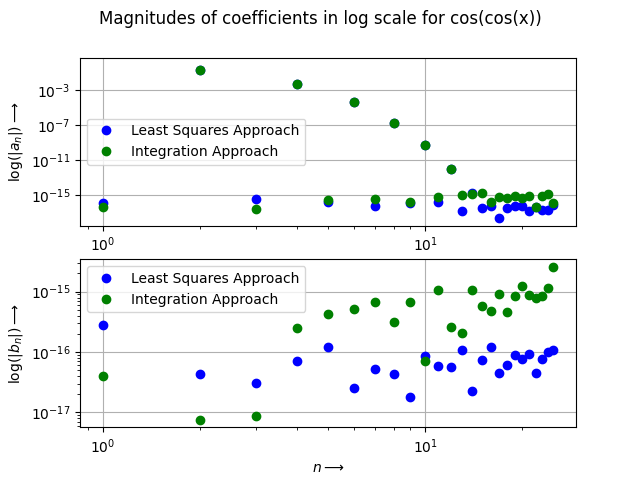
\includegraphics[scale = 0.7]{Q5-4.png}
    \caption{$cos(cos(x))\ in\ loglog\ scale$}
    \label{fig:Figure 10}
\end{figure}

\newpage
\section{Difference between the two methods}
\par We can clearly see that the difference in coefficients between the two methods is much more in $e^x$ than in $cos(cos(x))$. This is due to the fact that our definition of $e^x$ is discontinious and thus this error is much more accountable in integration method than in least square method.
\par If we find the maximum error between the two methods, we get \\
\begin{lstlisting}
#Calculating max error in the two methods
error_exp = np.abs(coeffs_exp - coeffs_exp_lstsq)
error_coscos = np.abs(coeffs_coscos - coeffs_coscos_lstsq)
max_error_exp = np.max(error_exp)
max_error_coscos = np.max(error_coscos)

print("Maximum error between the two methods for e^x is ",max_error_exp)
print("Maximum error between the two methods for cos(cos(x)) is ",max_error_coscos)
\end{lstlisting}
Maximum error between the two methods for $e^x$ is  1.332730870335368\\
Maximum error between the two methods for cos(cos(x)) is  2.68042108650032e-15\\



\section{Convergence to actual function}
\par Using the predicted values of the fourier coefficients, we can calculate the functional values for both $e^x$ and $cos(cos(x))$ by multiplying our coefficient vector with the earlier defined matrix A.
\begin{lstlisting}
#Plotting graph obtained from fourier coefficients alongside the original graph
def plotting_convergence():
    fourier_exp = np.matmul(A,coeffs_exp_lstsq)
    fourier_coscos = np.matmul(A,coeffs_coscos_lstsq)

    #e^x
    figure(11)
    semilogy(fourier_exp, 'm', label = 'Fourier representation')
    semilogy(generate_perodic_exp(x), 'c', label = 'Original function')
    grid(True)
    title(r'Convergence of Fourier Series representation to actual function for e^x')
    xlabel(r'$x\longrightarrow$')
    ylabel(r'Value in log scale$\longrightarrow$')
    legend()
    savefig("Q7-1.png")
    close()

    #cos(cos(x))
    figure(12)
    semilogy(fourier_coscos, 'm', label = 'Fourier representation')
    semilogy(generate_coscos(x), 'b', label = 'Original function')
    grid(True)
    title(r'Convergence of Fourier Series representation to actual function for cos(cos(x))', fontsize = 10)
    xlabel(r'$x\longrightarrow$')
    ylabel(r'Value in log scale$\longrightarrow$', fontsize = 8)
    legend()
    savefig("Q7-2.png")
    close()
    
plotting_convergence()      #Q7 plots function call
\end{lstlisting}
\begin{figure}[!tbh]
    \centering
    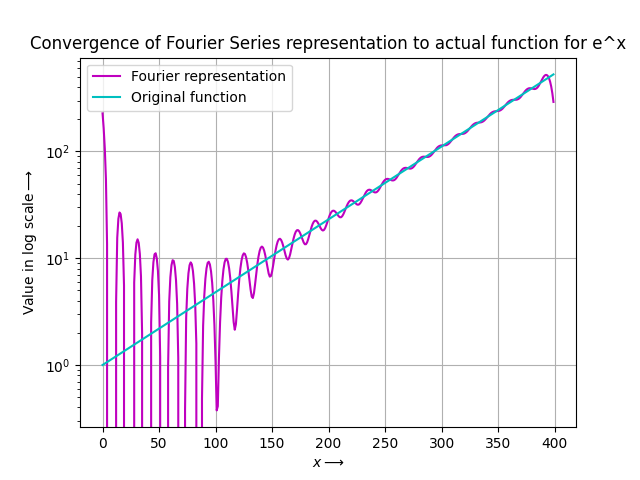
\includegraphics[scale = 0.7]{Q7-1.png}
    \caption{$e^x$}
    \label{fig:Figure 11}
\end{figure}
\begin{figure}[!tbh]
    \centering
    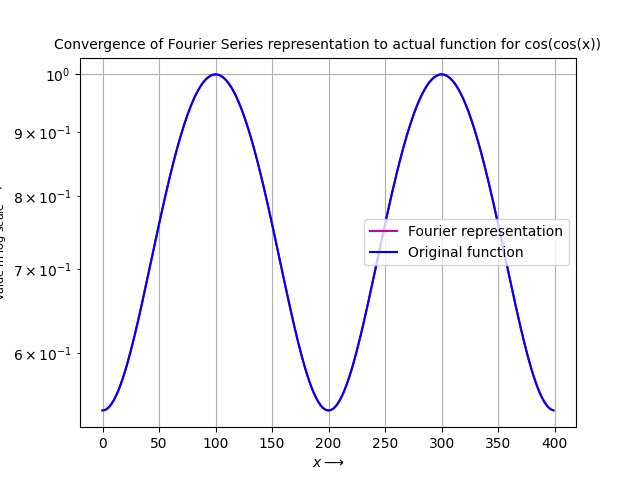
\includegraphics[scale = 0.7]{Q7-2.png}
    \caption{$cos(cos(x))$}
    \label{fig:Figure 12}
\end{figure}
\par We can clearly see from Figure \ref{fig:Figure 12} as well that the fourier representation of $cos(cos(x))$ is perfectly overlapping with the actual curve. However, from Figure \ref{fig:Figure 11}, we see that there is a huge deviation in the case of $e^x$. The main cause of this is that, to perfectly account for the discontinuities in $e^x$ we need infinite harmonics whereas we are only considering 51 coefficients. However this is not the case for $cos(cos(x))$, which because it is sinusodial in nature, is very nicely fit by even just 51 fourier coefficients.

\section{Conclusion}
\par In this assignment, we learnt how to calculate the fourier series coefficients for a perodic function by two methods, namely integration and least square.
\par Also, we saw that as our $e^x$ was discontinious, there was significant error between the curve we predicted and the actual curve. Whereas that was not the case for $cos(cos(x))$.
\end{document}
